\documentclass[11pt]{article}
\usepackage[margin=1in]{geometry}
\usepackage{graphicx}
\usepackage{booktabs}
\usepackage{caption}
\usepackage{xcolor}
\usepackage{hyperref}
\hypersetup{colorlinks=true, linkcolor=blue!50!black, citecolor=blue!50!black, urlcolor=blue!50!black}
\usepackage{microtype}
\usepackage{amsmath, amssymb}

\usepackage{tikz}
\usetikzlibrary{arrows.meta, shapes.geometric, shapes.symbols, positioning, calc, fit}
% Shared TikZ styles for architecture diagrams.
% Inputted from report.tex preamble *after* \usepackage{tikz} and the
% libraries arrows.meta / shapes.geometric / shapes.symbols / positioning / calc.
\tikzset{
  >=Stealth,
  data/.style    = {draw, circle, minimum size=6.2mm, fill=blue!10,
                    font=\scriptsize, inner sep=1pt},
  enc/.style     = {draw, semicircle, shape border rotate=0,
                    minimum width=8mm, minimum height=4mm, inner sep=1pt,
                    fill=orange!30, font=\scriptsize},
  frozen/.style  = {draw, semicircle, shape border rotate=0,
                    minimum width=9mm, minimum height=4.5mm, inner sep=1pt,
                    fill=cyan!18, font=\scriptsize},
  pred/.style    = {draw, rounded rectangle,
                    minimum width=9mm, minimum height=5mm, inner sep=2pt,
                    fill=green!28, font=\scriptsize},
  loss/.style    = {draw, rectangle, minimum size=5mm, fill=yellow!45,
                    font=\scriptsize, inner sep=2pt},
  op/.style      = {draw, rectangle, rounded corners=1pt,
                    minimum width=11mm, minimum height=5mm, inner sep=2pt,
                    fill=gray!12, font=\scriptsize, align=center},
  block/.style   = {draw, rounded corners=2pt,
                    minimum width=12mm, minimum height=8mm, inner sep=2pt,
                    fill=blue!12, font=\scriptsize, align=center},
  attn/.style    = {block, fill=red!15},
  meta/.style    = {font=\tiny, gray!75, inner sep=1pt},
  arrow/.style   = {->, semithick},
  noarrow/.style = {->, semithick, dashed, gray!75},
}


\graphicspath{{../data/figures/}}

\title{JEPA Pretraining for Physical Parameter Regression\\
       \large Empirical Study on \texttt{active\_matter}}

\newcommand{\probe}[1]{\textsc{#1}}
\newcommand{\code}[1]{\texttt{#1}}

\begin{document}
\maketitle

\section{Introduction}

We pretrain a video encoder on \texttt{active\_matter} simulations from
\href{https://github.com/PolymathicAI/the_well}{The~Well} using a JEPA-style
self-supervised objective, then evaluate the frozen features by regressing the
underlying physical parameters $(\alpha, \zeta)$ with three probes of
increasing capacity: a linear probe (\probe{linear}), a $k$-NN probe with a
sweep over $k$ and metric (\probe{knn}), and an attentive probe
(\probe{attentive}). We report validation MSE in z-score units; lower is
better. The headline question is which design decisions actually move the
needle, not whether any single number is state-of-the-art.

\section{Experimental setup}

\paragraph{Data.} \texttt{active\_matter} samples are 16-frame clips, native
$256{\times}256$. Each (context, target) JEPA window draws a single sample
$(\alpha, \zeta)$ as the regression label.

\paragraph{Pretraining.} The encoder is a pure 3D-conv ResNet
(\code{conv3d\_next}) with optional self-attention stages, or a 3D ViT
(\code{vit3d}). The objective is VICReg-style invariance$+$variance$+$covariance
on context/target embeddings unless noted otherwise. Each pretraining run is
followed by per-checkpoint probe evaluation, and an aggregate \emph{eval-curve}
run that re-runs all three probes at every checkpoint and writes one tidy log.

\paragraph{Probes.}
\begin{itemize}
  \item \probe{linear}: closed-form least-squares on z-normalised features.
  \item \probe{knn}: best of a sweep over $k \in \{1, 5, 10, 20, 50\}$ and
        $\{$cosine, Euclidean$\}$. Only the swept best mean MSE is logged
        per epoch.
  \item \probe{attentive}: a small cross-attention pooler on top of the
        frozen feature tokens, trained to convergence per checkpoint.
\end{itemize}

The linear and $k$-NN probes share the encode-then-pool front end shown in
Figures~\ref{fig:linear-probe} and~\ref{fig:knn-probe}; only the head differs.

\begin{figure}[h]
\centering
% Linear probe: frozen encoder -> spatial pool -> closed-form ridge regression.
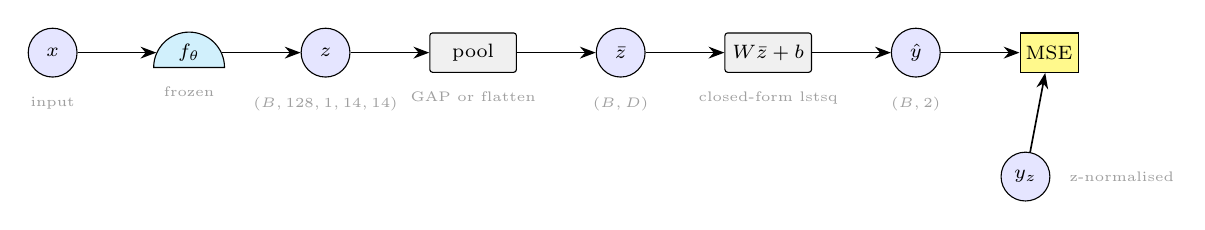
\begin{tikzpicture}[
  node distance = 5mm and 10mm,
  every node/.style = {font=\scriptsize, inner sep=1.5pt}]

  \node[data]                  (x)    {$x$};
  \node[frozen, right=of x]    (enc)  {$f_{\theta}$};
  \node[data, right=of enc]    (z)    {$z$};
  \node[op,   right=of z]      (pool) {pool};
  \node[data, right=of pool]   (zb)   {$\bar z$};
  \node[op,   right=of zb]     (W)    {$W\bar z + b$};
  \node[data, right=of W]      (yh)   {$\hat y$};
  \node[loss, right=of yh]     (mse)  {MSE};
  \node[data, below=10mm of mse, xshift=-3mm] (y)   {$y_{z}$};

  \foreach \a/\b in {x/enc, enc/z, z/pool, pool/zb, zb/W, W/yh, yh/mse}
    \draw[arrow] (\a) -- (\b);
  \draw[arrow] (y) -- (mse);

  \node[meta, below=2mm of x]    {input};
  \node[meta, below=2mm of enc]  {frozen};
  \node[meta, below=2mm of z]    {$(B,128,1,14,14)$};
  \node[meta, below=2mm of pool] {GAP or flatten};
  \node[meta, below=2mm of zb]   {$(B,D)$};
  \node[meta, below=2mm of W]    {closed-form lstsq};
  \node[meta, below=2mm of yh]   {$(B,2)$};
  \node[meta, right=2mm of y, font=\tiny, gray!75] {z-normalised};
\end{tikzpicture}

\caption{Linear probe. The encoder is frozen (cyan); features $z$ are
  spatially pooled (\code{feature\_pool}\,$\in\,\{$\code{gap}, \code{flatten}$\}$)
  into $\bar z\!\in\!\mathbb R^D$ and a closed-form least-squares fit
  predicts the z-normalised parameter vector $\hat y\!=\!W\bar z + b$.
  No SGD; the regulariser is the implicit minimum-norm solution.}
\label{fig:linear-probe}
\end{figure}

\begin{figure}[h]
\centering
% k-NN probe: query vs training memory bank, both encoded by the same frozen f_theta.
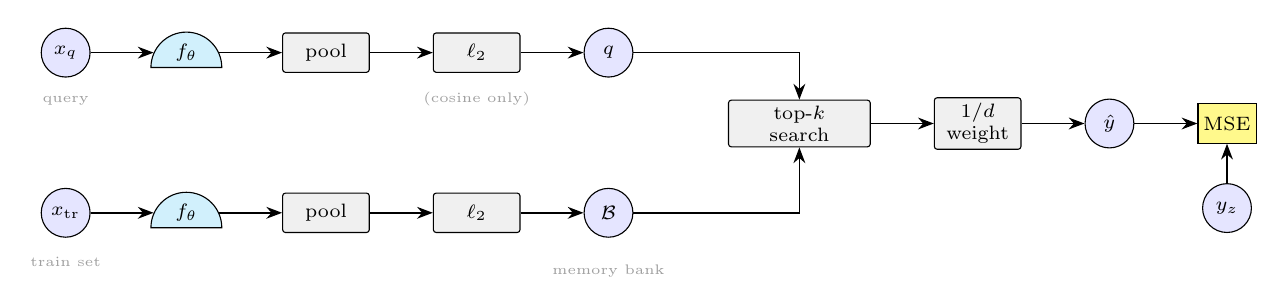
\begin{tikzpicture}[
  node distance = 5mm and 8mm,
  every node/.style = {font=\scriptsize, inner sep=1.5pt}]

  % Top row: query path
  \node[data]                       (xq)   {$x_q$};
  \node[frozen, right=of xq]        (enc)  {$f_{\theta}$};
  \node[op,   right=of enc]         (pool) {pool};
  \node[op,   right=of pool]        (norm) {$\ell_{2}$};
  \node[data, right=of norm]        (q)    {$q$};

  % Bottom row: memory bank
  \node[data, below=14mm of xq]     (xt)   {$x_{\mathrm{tr}}$};
  \node[frozen, right=of xt]        (enc2) {$f_{\theta}$};
  \node[op,   right=of enc2]        (pool2){pool};
  \node[op,   right=of pool2]       (norm2){$\ell_{2}$};
  \node[data, right=of norm2]       (B)    {$\mathcal{B}$};

  % Right column: search and prediction (vertically centred between rows)
  \node[op, right=12mm of q, yshift=-9mm,
        minimum width=18mm, align=center]   (knn) {top-$k$\\search};
  \node[op, right=of knn, align=center]     (idw) {$1/d$\\weight};
  \node[data, right=of idw]                 (yh)  {$\hat y$};
  \node[loss, right=of yh]                  (mse) {MSE};
  \node[data, below=of mse]                 (y)   {$y_z$};

  % Edges
  \foreach \a/\b in {xq/enc, enc/pool, pool/norm, norm/q,
                     xt/enc2, enc2/pool2, pool2/norm2, norm2/B}
    \draw[arrow] (\a) -- (\b);
  \draw[arrow] (q) -| (knn.north);
  \draw[arrow] (B) -| (knn.south);
  \draw[arrow] (knn) -- (idw);
  \draw[arrow] (idw) -- (yh);
  \draw[arrow] (yh)  -- (mse);
  \draw[arrow] (y)   -- (mse);

  % Annotations
  \node[meta, below=2mm of xq]   {query};
  \node[meta, below=2mm of xt]   {train set};
  \node[meta, below=2mm of norm] {(cosine only)};
  \node[meta, below=2mm of B, yshift=-1mm] {memory bank};
\end{tikzpicture}

\caption{$k$-NN probe. The query $x_q$ and every training sample
  $x_{\mathrm{tr}}$ pass through the same frozen encoder and pool, producing
  the query feature $q$ and a memory bank $\mathcal{B}$. For the cosine
  metric both are $\ell_2$-normalised; for Euclidean they are not. We sweep
  $k\!\in\!\{1,5,10,20,50\}$ and $d\!\in\!\{$Euclidean, cosine$\}$; the $k$
  nearest training points contribute to $\hat y$ with inverse-distance
  weights, and the best $(k, d)$ mean MSE is logged per checkpoint.}
\label{fig:knn-probe}
\end{figure}

\section{From the original baseline to a stable training recipe}

The original recipe (\href{https://wandb.ai/ry2665-new-york-university/physics-jepa-baseline/runs/ztffyvmc}{run \code{ztffyvmc}})
used batch size 8 and fp32 on a single A100, following the JEPA literature.
Training repeatedly out-of-memoried; we dropped to batch size 2 to fit, but
VICReg's invariance term is famously sensitive to small batches and
representations collapsed by mid-training. Switching to bf16 freed enough
memory to restore batch size 8
(\href{https://wandb.ai/ry2665-new-york-university/physics-jepa-baseline/runs/6mhmw4k6}{run \code{6mhmw4k6}});
this is what we call the \emph{baseline} below.

\begin{figure}[h]
  \centering
  \includegraphics[width=0.85\textwidth]{fig_linear_mean.pdf}
  \caption{\probe{linear} mean MSE vs.\ pretrain epoch. The bs$=$2 run
    (grey, dashed) descends, then degrades past epoch 11 — the hallmark of
    VICReg collapse with too small a batch. The bs$=$8 bf16 baseline (blue)
    converges to $0.243$, a $21\%$ improvement on the bs$=$2 best
    ($0.308$). ViT3D (purple) is roughly $3\times$ better than every CNN
    variant.}
  \label{fig:linear-mean}
\end{figure}

The same pattern shows up for \probe{attentive} (Figure~\ref{fig:attentive-mean}):
the bs$=$2 attentive curve actually \emph{climbs} after epoch 11, while the
bs$=$8 baseline holds its minimum and the FFT runs slightly improve on it.

\begin{figure}[h]
  \centering
  \includegraphics[width=0.85\textwidth]{fig_attentive_mean.pdf}
  \caption{\probe{attentive} mean MSE vs.\ pretrain epoch. Conv$+$Attn (FFT)
    reaches the lowest attentive MSE ($0.072$ at epoch 13). ViT3D is omitted
    here because its attentive probe runs crashed before logging.}
  \label{fig:attentive-mean}
\end{figure}

\section{FFT preprocessing replaces the per-dataset crop}

The default loader crops each frame to a square that fits the model's stride;
on \texttt{active\_matter} this is the native $256{\times}256$ but on the
other Well datasets it discards information. We replaced the crop with a
band-limited FFT resize that preserves periodic boundary conditions
(\href{https://wandb.ai/ry2665-new-york-university/physics-jepa-baseline/runs/5b2obx5w}{run \code{5b2obx5w}}).
The pipeline is shown in Figure~\ref{fig:fft-pipeline}: the native frame is
transformed to the frequency domain, the spectrum is centred and either
centre-cropped (downsample) or zero-padded (upsample) to the target size,
then inverse-transformed and re-scaled by $\rho = HW / H_n W_n$ so amplitude
is preserved. Even on a dataset where there is nothing to crop, FFT still
gave a small but consistent win: linear $0.243 \to 0.212$, k-NN
$0.217 \to 0.174$, attentive $0.081 \to 0.079$. Every subsequent experiment
uses FFT.

\begin{figure}[h]
\centering
% FFT-based resize pipeline (resize_mode: fft).
% Adds tiny spatial- / frequency-domain thumbnails so the reader can see
% what each step does to the data.
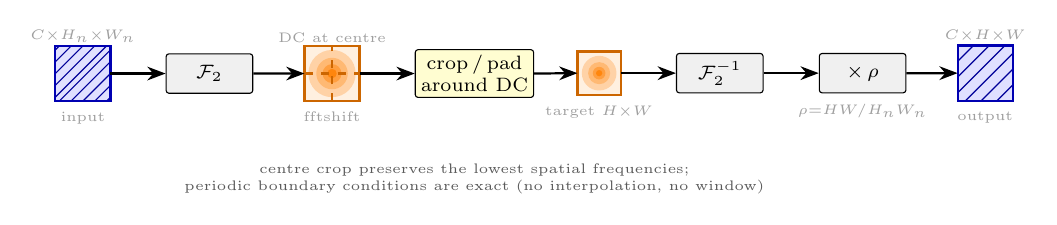
\begin{tikzpicture}[
  node distance = 4mm and 7mm,
  every node/.style = {font=\scriptsize, inner sep=1.5pt}]

  % ---------- thumbnail helper styles --------------------------------
  % spatial-domain thumbnail: a few diagonal "wave" stripes
  % frequency-domain thumbnail: a centred bright DC bin with a faint halo

  % ---------- input spatial thumbnail --------------------------------
  \begin{scope}[local bounding box=xthumb]
    \fill[blue!12] (0,0) rectangle (0.7,0.7);
    \foreach \k in {0.05, 0.20, 0.35, 0.50, 0.65} {
      \draw[blue!60!black, thin] (0,\k) -- (0.7-\k, 0.7);
      \draw[blue!60!black, thin] (\k, 0) -- (0.7, 0.7-\k);
    }
    \draw[draw=blue!70!black, thick] (0,0) rectangle (0.7,0.7);
  \end{scope}
  \node[meta, below=1mm of xthumb] {input};
  \node[meta, above=0mm of xthumb] {$C{\times}H_n{\times}W_n$};
  % ---------- F2: full spectrum thumbnail ----------------------------
  \node[op, right=of xthumb] (fft) {$\mathcal{F}_{2}$};
  \begin{scope}[local bounding box=spec1, shift={($(fft.east) + (0.65, -0.35)$)}]
    \fill[orange!12] (0,0) rectangle (0.7,0.7);
    % bright DC bin + halo
    \foreach \r/\op in {0.30/35, 0.20/55, 0.12/75, 0.06/95} {
      \fill[orange!\op] (0.35,0.35) circle (\r);
    }
    \draw[orange!80!black, thick, dashed] (0.35,0) -- (0.35,0.7);
    \draw[orange!80!black, thick, dashed] (0,0.35) -- (0.7,0.35);
    \draw[draw=orange!80!black, thick] (0,0) rectangle (0.7,0.7);
  \end{scope}
  \node[meta, below=1mm of spec1] {fftshift};
  \node[meta, above=0mm of spec1] {DC at centre};
  \draw[arrow, thick] (xthumb.east) -- (fft.west);
  \draw[arrow, thick] (fft.east) -- ($(spec1.west) + (0,0.0)$);

  % ---------- crop / pad ---------------------------------------------
  \node[op, right=of spec1, align=center, fill=yellow!18] (cp)
    {crop\,/\,pad\\around DC};
  \begin{scope}[local bounding box=spec2,
                shift={($(cp.east) + (0.55, -0.27)$)}]
    \fill[orange!12] (0,0) rectangle (0.55,0.55);
    \foreach \r/\op in {0.22/35, 0.14/55, 0.08/75, 0.04/95} {
      \fill[orange!\op] (0.275,0.275) circle (\r);
    }
    \draw[draw=orange!80!black, thick] (0,0) rectangle (0.55,0.55);
  \end{scope}
  \draw[arrow, thick] (spec1.east) -- (cp.west);
  \draw[arrow, thick] (cp.east) -- ($(spec2.west) + (0,0)$);
  \node[meta, below=1mm of spec2] {target $H{\times}W$};

  % ---------- ifftshift, F2^-1, scale --------------------------------
  \node[op, right=of spec2] (ift) {$\mathcal{F}_{2}^{-1}$};
  \node[op, right=of ift,  align=center] (sc)  {$\times\,\rho$};
  \node[meta, below=1mm of sc] {$\rho{=}HW/H_nW_n$};

  % ---------- output spatial thumbnail -------------------------------
  \begin{scope}[local bounding box=ythumb,
                shift={($(sc.east) + (0.65, -0.35)$)}]
    \fill[blue!12] (0,0) rectangle (0.7,0.7);
    \foreach \k in {0.10, 0.30, 0.50} {
      \draw[blue!60!black, thin] (0,\k) -- (0.7-\k, 0.7);
      \draw[blue!60!black, thin] (\k, 0) -- (0.7, 0.7-\k);
    }
    \draw[draw=blue!70!black, thick] (0,0) rectangle (0.7,0.7);
  \end{scope}
  \node[meta, below=1mm of ythumb] {output};
  \node[meta, above=0mm of ythumb] {$C{\times}H{\times}W$};
  \draw[arrow, thick] (spec2.east) -- (ift.west);
  \draw[arrow, thick] (ift.east) -- (sc.west);
  \draw[arrow, thick] (sc.east) -- ($(ythumb.west) + (0,0)$);

  % bottom note
  \node[meta, below=8mm of cp, align=center, gray!70!black]
    {centre crop preserves the lowest spatial frequencies;\\
     periodic boundary conditions are exact (no interpolation, no window)};
\end{tikzpicture}

\caption{FFT-based resize (\code{resize\_mode: fft}). $\mathcal{F}_2$ is the
  2-D Fourier transform; the centre crop or zero-pad happens around the DC
  bin so the lowest spatial frequencies are preserved and aliasing is exact.
  Periodic boundary conditions are exact (no interpolation or window).}
\label{fig:fft-pipeline}
\end{figure}

\begin{figure}[h]
  \centering
  \includegraphics[width=0.85\textwidth]{fig_knn_mean.pdf}
  \caption{\probe{knn} mean MSE vs.\ pretrain epoch (best $k$ and metric per
    epoch). The FFT run (orange) opens a clear gap on the bilinear baseline
    after epoch 13. ViT3D continues to improve past epoch 25, the only
    architecture that does so.}
  \label{fig:knn-mean}
\end{figure}

\section{Architectural variants}

Building on the FFT recipe, we ran three variants.

\paragraph{Conv$+$Attn.}
A self-attention block after the last 3D-conv stage
(\href{https://wandb.ai/ry2665-new-york-university/physics-jepa-baseline/runs/ih2xhy8w}{run \code{ih2xhy8w}}).
The architecture (Figure~\ref{fig:conv-attn}) is identical to the default
\code{conv3d\_next} backbone used by the bilinear and FFT runs through all
four stages; a single transformer block with 4 heads and MLP ratio 4 is
appended at stage 4. Slightly improves linear ($0.207$) and gives the best
attentive MSE of any CNN variant ($0.072$).

\begin{figure}[h]
\centering
% conv3d_next_attn encoder.
% Two-row layout that mirrors ViT3D, with the key visual contrast:
% the post-conv tensor is drawn as a flat spatial grid (no depth)
% so it is visually obvious that the attention has only spatial
% structure to mix — there is no temporal axis left to act on.
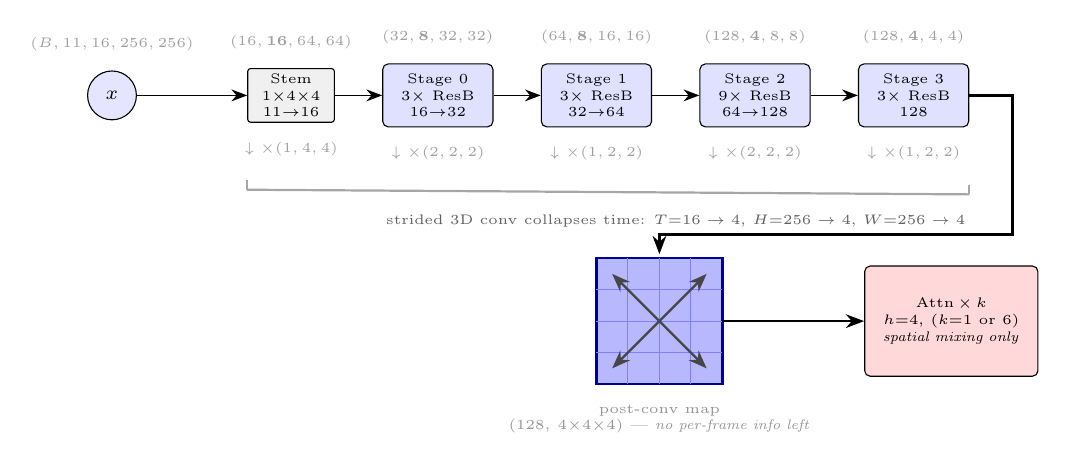
\begin{tikzpicture}[
  node distance = 6mm and 6mm,
  every node/.style = {font=\scriptsize, inner sep=1.5pt}]

  % =====================================================================
  % ROW 1: pipeline
  % =====================================================================
  \node[data]                                                   (x)    {$x$};
  \node[op,    right=14mm of x, align=center, font=\tiny]       (stem) {Stem\\$1{\times}4{\times}4$\\$11{\to}16$};
  \node[block, right=of stem, align=center, font=\tiny, minimum width=14mm] (s0) {Stage 0\\$3{\times}$ ResB\\$16{\to}32$};
  \node[block, right=of s0,   align=center, font=\tiny, minimum width=14mm] (s1) {Stage 1\\$3{\times}$ ResB\\$32{\to}64$};
  \node[block, right=of s1,   align=center, font=\tiny, minimum width=14mm] (s2) {Stage 2\\$9{\times}$ ResB\\$64{\to}128$};
  \node[block, right=of s2,   align=center, font=\tiny, minimum width=14mm] (s3) {Stage 3\\$3{\times}$ ResB\\$128$};

  \foreach \a/\b in {x/stem, stem/s0, s0/s1, s1/s2, s2/s3}
    \draw[arrow] (\a) -- (\b);

  \node[meta, above=2mm of x]    {$(B,11,16,256,256)$};
  \node[meta, above=2mm of stem] {$(16,\mathbf{16},64,64)$};
  \node[meta, above=2mm of s0]   {$(32,\mathbf{8},32,32)$};
  \node[meta, above=2mm of s1]   {$(64,\mathbf{8},16,16)$};
  \node[meta, above=2mm of s2]   {$(128,\mathbf{4},8,8)$};
  \node[meta, above=2mm of s3]   {$(128,\mathbf{4},4,4)$};

  \node[meta, below=2mm of stem] {$\downarrow{\times}(1,4,4)$};
  \node[meta, below=2mm of s0]   {$\downarrow{\times}(2,2,2)$};
  \node[meta, below=2mm of s1]   {$\downarrow{\times}(1,2,2)$};
  \node[meta, below=2mm of s2]   {$\downarrow{\times}(2,2,2)$};
  \node[meta, below=2mm of s3]   {$\downarrow{\times}(1,2,2)$};

  % T axis collapse highlight
  \draw[thick, gray!70]
    ($(stem.south west) + (0, -0.85)$) --
    ($(s3.south east) + (0, -0.85)$);
  \draw[thick, gray!70]
    ($(stem.south west) + (0, -0.85)$) -- ++(0, 0.12);
  \draw[thick, gray!70]
    ($(s3.south east) + (0, -0.85)$) -- ++(0, 0.12);
  \node[font=\tiny, gray!75!black, align=center, anchor=north]
    at ($(s1.south east)!0.5!(s2.south west) + (0, -1.05)$)
    {strided 3D conv collapses time:
     $T{=}16 \to 4$, $H{=}256 \to 4$, $W{=}256 \to 4$};

  % =====================================================================
  % ROW 2: a flat 4x4 spatial grid -- "no temporal info left"
  % =====================================================================
  \node[below=32mm of s1.south] (grid_anchor) {};

  % single flat plane representing the post-conv tensor.
  % (4 t'-slices collapsed visually into one plane to emphasize that
  % the temporal axis carries no usable information.)
  \begin{scope}[local bounding box=grid]
    \draw[fill=blue!28, draw=blue!60!black, thick]
      ($(grid_anchor)$) rectangle ++(1.6, 1.6);
    \foreach \g in {0.4, 0.8, 1.2} {
      \draw[blue!50, thin] ($(grid_anchor) + (\g, 0)$) -- ++(0, 1.6);
      \draw[blue!50, thin] ($(grid_anchor) + (0, \g)$) -- ++(1.6, 0);
    }
    % a few in-plane (purely spatial) attention edges
    \draw[<->, thick, gray!55!black]
      ($(grid_anchor) + (0.20, 0.20)$) --
      ($(grid_anchor) + (1.40, 1.40)$);
    \draw[<->, thick, gray!55!black]
      ($(grid_anchor) + (0.20, 1.40)$) --
      ($(grid_anchor) + (1.40, 0.20)$);
  \end{scope}
  \node[font=\tiny, gray!85, align=center, below=2mm of grid]
    {post-conv map\\$(128,\,4{\times}4{\times}4)$ — \emph{no per-frame info left}};

  % connector: right of Stage 3 -> down past the caption -> left ->
  % down onto the post-conv grid. Routed around the right side so it
  % does not cross the brace caption.
  \coordinate (c1) at ($(s3.east) + (0.55, 0)$);
  \coordinate (c3) at ($(grid.north) + (0, 0.30)$);
  \coordinate (c2) at (c1 |- c3);
  \draw[arrow, thick]
    (s3.east) -- (c1) -- (c2) -- (c3) -- ($(grid.north) + (0, 0.05)$);

  % attention block (no z output — diagram stops at attention)
  \node[attn, right=18mm of grid.east, align=center, font=\tiny,
        minimum width=22mm, minimum height=14mm]
    (att) {Attn$\,\times\,k$\\$h{=}4$, ($k{=}1$ or $6$)\\\textit{spatial mixing only}};
  \draw[arrow, thick] (grid.east) -- (att.west);

\end{tikzpicture}

\caption{Conv$+$Attn encoder (\code{conv3d\_next\_attn} with
  \code{attn\_stages:[4]}). Channel progression $16{\to}32{\to}64{\to}128{\to}128$,
  total $16{\times}$ spatial stride, time stride $4{\times}$. Stride
  annotations show $(\Delta T, \Delta H, \Delta W)$ at each stage. The red
  attention block is the only structural difference from the default conv
  backbone used by the bilinear and FFT runs.}
\label{fig:conv-attn}
\end{figure}

\paragraph{ViT3D.}
A 3D-patch ViT with depth 6 (Figure~\ref{fig:vit3d}; group
\code{...vit3d-depth6\_2026-04-25\_11-11-48}). It dominates both
\probe{linear} ($0.086$) and \probe{knn} ($0.081$) by a wide margin, but
HPC-quota exhaustion meant we could only run per-checkpoint frozen probes;
the aggregate eval-curve runs and the attentive probe crashed
mid-execution. The ViT3D points in
Figures~\ref{fig:linear-mean}--\ref{fig:knn-mean} are the per-checkpoint
summary values stitched into a curve.

\begin{figure}[h]
\centering
% ViT3D depth-6 encoder.
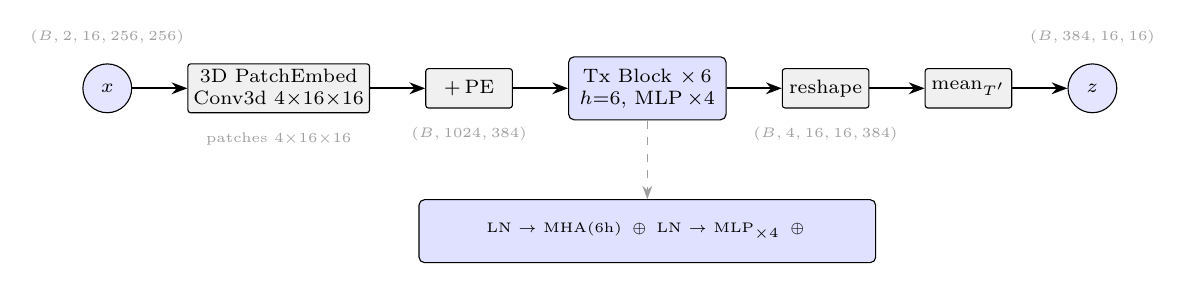
\begin{tikzpicture}[
  node distance = 6mm and 7mm,
  every node/.style = {font=\scriptsize, inner sep=1.5pt}]

  \node[data]                                                   (x)   {$x$};
  \node[op,   right=of x,  minimum width=20mm, align=center]    (pe)  {3D PatchEmbed\\Conv3d $4{\times}16{\times}16$};
  \node[op,   right=of pe, align=center]                        (pos) {$+\,\mathrm{PE}$};
  \node[block, right=of pos, minimum width=20mm, align=center]  (blk) {Tx Block $\times\,6$\\$h{=}6$, MLP$\,{\times}4$};
  \node[op,   right=of blk, align=center]                       (rs)  {reshape};
  \node[op,   right=of rs,  align=center]                       (mt)  {mean$_{T'}$};
  \node[data, right=of mt]                                      (z)   {$z$};

  \foreach \a/\b in {x/pe, pe/pos, pos/blk, blk/rs, rs/mt, mt/z}
    \draw[arrow] (\a) -- (\b);

  \node[meta, above=2mm of x]   {$(B,2,16,256,256)$};
  \node[meta, above=2mm of z]   {$(B,384,16,16)$};
  \node[meta, below=2mm of pe]  {patches $4{\times}16{\times}16$};
  \node[meta, below=2mm of pos] {$(B,1024,384)$};
  \node[meta, below=2mm of rs]  {$(B,4,16,16,384)$};

  % Block internals shown beneath
  \node[block, below=10mm of blk, minimum width=58mm,
        align=center, font=\tiny]
    (blkin) {LN $\to$ MHA(6h) $\,\oplus\,$ LN $\to$ MLP$_{\times 4}$ $\,\oplus\,$};
  \draw[noarrow, thin] (blk.south) -- (blkin.north);
\end{tikzpicture}

\caption{ViT3D depth-6 encoder. A single 3D convolution patches the input
  into a $4{\times}16{\times}16$ grid of $384$-dim tokens; the flattened
  $1024$ tokens go through six pre-norm transformer blocks (heads $h{=}6$,
  MLP ratio $4$). Time is folded back by reshaping and averaging over $T'$
  to yield a $(B, 384, 16, 16)$ feature map matched to the predictor.}
\label{fig:vit3d}
\end{figure}

\paragraph{SIGReg.}
A LeWM-style alternative regulariser
(\href{https://wandb.ai/ry2665-new-york-university/physics-jepa-baseline/runs/wbo7xqs0}{run \code{wbo7xqs0}}).
The training loss did not converge; the probe MSE \emph{rises} during
pretraining
(Figures~\ref{fig:linear-mean} and \ref{fig:knn-mean}, red dotted), so
the best probe scores happen at epoch 1 before the encoder collapses. We
keep it in the figures as a negative control and do not analyse it
further.

\section{Per-parameter difficulty}

\begin{figure}[h]
  \centering
  \includegraphics[width=0.78\textwidth]{fig_per_param_best.pdf}
  \caption{Linear-probe MSE on $\alpha$ (top) vs.\ $\zeta$ (bottom).
    $\zeta$ is consistently $\sim$$5$--$50\times$ harder than $\alpha$,
    and the gap is largest for the CNN family — ViT3D narrows it the
    most ($\zeta = 0.167$ vs.\ $\alpha = 0.004$).}
  \label{fig:per-param}
\end{figure}

Splitting MSE by parameter (Figure~\ref{fig:per-param}) is the clearest
single visualisation of where the remaining error lives: $\alpha$ is
nearly solved (linear $\alpha$ MSE drops below $0.01$ for ViT3D), while
$\zeta$ remains in the $0.17$--$0.42$ range. Future work that wants to
chase the next absolute improvement should focus on $\zeta$.

\section{Summary}

\begin{figure}[h]
  \centering
  \includegraphics[width=0.95\textwidth]{fig_best_summary_bars.pdf}
  \caption{Best validation MSE per (config, probe). Lower is better. The
    Conv$+$Attn run wins on attentive; ViT3D wins on linear and k-NN by a
    wide margin. Attentive bars are absent for SIGReg (no probe was run on
    that group) and ViT3D (probe crashed).}
  \label{fig:bars}
\end{figure}

\begin{table}[h]
  \centering
  \small
  \begin{tabular}{lrrrrr}
    \toprule
    Config & Linear & k-NN & Attentive & Best $\alpha$ & Best $\zeta$ \\
    \midrule
    VICReg, bs$=$2 (fp32)            & 0.308 & 0.232 & 0.134 & 0.091 & 0.178 \\
    VICReg, bs$=$8 (bf16) [baseline] & 0.243 & 0.217 & 0.081 & 0.028 & 0.135 \\
    VICReg + FFT preproc             & 0.212 & 0.174 & 0.079 & 0.028 & 0.129 \\
    Conv+Attn (FFT)                  & 0.207 & 0.184 & \textbf{0.072} & 0.028 & 0.116 \\
    SIGReg (FFT, did not converge)   & 0.599 & 0.478 & ---   & 0.227 & 0.729 \\
    ViT3D-d6 (FFT)                   & \textbf{0.086} & \textbf{0.081} & --- & \textbf{0.005} & \textbf{0.167} \\
    \bottomrule
  \end{tabular}
  \caption{Best mean / per-parameter validation MSE for each configuration
    (lower is better). Linear/k-NN/Attentive columns are the
    \texttt{best\_mean} from the eval-curve run. The two right columns are
    the best $\alpha$ and $\zeta$ achieved by the linear probe. Bold marks
    the best per column among converged runs. ViT3D's $\zeta$ is best on
    the linear probe but its $\zeta$ value is only modestly lower than the
    CNN family — the $\alpha$ improvement is what moves its mean.}
  \label{tab:summary}
\end{table}

The takeaways:
\begin{enumerate}
  \item bf16$+$bs$=$8 is a strict prerequisite. fp32$+$bs$=$2 collapses.
  \item FFT preprocessing helps even on a dataset whose native size already
        matches the model — likely because the resize preserves periodic
        boundary conditions.
  \item Adding self-attention to the conv backbone is a low-risk win on the
        attentive probe.
  \item ViT3D is the most promising backbone we tried. The remaining
        question is whether its lead extrapolates to the other two Well
        datasets we have not yet trained on; that is left to future
        work, contingent on HPC quota.
  \item SIGReg in this configuration never converged. The negative result is
        documented but not analysed; see \href{https://wandb.ai/ry2665-new-york-university/physics-jepa-baseline/runs/wbo7xqs0}{wbo7xqs0}.
\end{enumerate}

\paragraph{Reproducibility.} All numbers and figures in this report are
produced by \code{data/fetch.py} and \code{data/plot.py}; running
\code{make all} from \code{data/} pulls every metric directly from
\href{https://wandb.ai/ry2665-new-york-university/physics-jepa-baseline}{wandb}
and re-renders the figures.

\end{document}
